%preamble
\documentclass[letterpaper]{article}
\synctex=1
\usepackage{graphicx}
\graphicspath{ {images/} }

\usepackage{lipsum}
\usepackage{float}
% \bibliographystyle{IEEEtran}
\bibliographystyle{ieeetr}

\usepackage{amssymb}

\usepackage{siunitx}
%actual document
\begin{document}

% \maketitle %insert titlepage here
\begin{titlepage}
 \begin{center}
  \vspace*{1cm}
  \Huge
  Experiment 4
  \vspace{1cm}

  Magnetic Forces
  \vspace{1cm}

  By: Arun Woosaree
  \vspace{1cm}

  Lab partners:
  \vspace{.25cm}
  \Large

  Fatemeh Ghafari Far\\
  % Purvish Jajal
  \vspace{.25cm}
  Yvonne Hong
  \vspace{1cm}

  \Huge
  PHYS 230 Lab EH71
  \vspace{1cm}

  TA: Andrei Tretiakov
  \vspace{1cm}

  Date of Lab: April 5, 2018%\today
  \vfill
 \end{center}
\end{titlepage}

\section{Introduction}
% Begin with experiment’s objectives\\
% Give physical background:\\
% ○ Describe investigated/used\\
% phenomena e.g. Gauss’s law,\\
% field lines, equipotential lines.\\
% ○ Do not copy text from a
% textbook/manual\\
% Provide equations you used\\
% ○ Identify all symbols\\
% \textbf{Equations for this lab}\\
% $$F_z(z)=-\frac{dU}{dz}$$
% $$U=-\mathbf{m}\cdot\mathbf{B}=-\mathbf{mB}\cos{\theta}$$
% $$U=-m_sB_m\cos{\theta}$$
% $$U=-\frac{m_s\mu_0m_m}{2\pi z^3}$$
% $$F_s=\pm \frac{3m_s\mu_0m_m}{2\pi z^4}=\pm\frac{3m_s\mu_0m_m}{2\pi}\frac{1}{z^4}$$
% $$\mathbf{m}=I\mathbf{A}$$
% $$\tao=\mathbf{m}\times\mathbf{B}=mb\sin{\theta}$$
% $$B_z=\frac{\mu_0Ia^2}{2(z^2+a^2)}$$
% \chi

In this experiment, we measure the forces on magnetic material from a strong permanent magnet,
which has an inhomogeneous magnetic field. From the force measurements, we are able to determine the type
of magnetic material. All materials fall into one of three magnetic classes.
Diamagnetic materials are weakly repelled by strong external magnets and paramagnetic materials are weakly attracted
regardless of the direction of the field, and quickly lose any magnetic moment when the external field is removed. Ferromagnetic materials are either `soft' or `hard'. Soft ferromagnets develop
a large net magnetic moment when an external field is applied but like paramagnetic and diamagnetic materials, the moment does not persist if the field is removed.
Hard ferromagnets retain a permanent magnetic dipole moment, even in the absence of an external field. They can be
strongly attracted, repelled and torqued by other magnets, depending on orientation.
We chose to measure the forces of a strong rare earth neodymium magnet (a hard ferromagnet) acting on
another hard ferromagnet, and a soft ferromagnet (a Canadian nickel).

We expect the force-distance power law for the main types of magnetic materials to be in the following format:
$$|F_m|=\frac{C}{z^n}, \hspace{1cm}n=4 \:or\: n=7,\hspace{0.5cm} C=some\:constants$$
For hard ferromagnetic samples, an inverse $4^{th}$ power law is predicted $(n=4)$, while for soft ferromagnets, and paramagnetic and diamagnetic materials,
an inverse $7^{th}$ power law is predicted. By analyzing the magnetic force of a strong neodymium magnet on our
samples at various distances, we experimentally confirm that a Canadian nickel is a soft ferromagnetic material, while
a common fridge magnet is a hard ferromagnetic material.

% \textbf{Spicy x: \chi}
\section{Experimental Method}
% List all equipment used\\
% ○ Provide parameters as detailed as
% possible: masses, frequencies,
% etc.\\
% Report what YOU DID to achieve
% experimental goals:\\
% ○ Do not use imperative clause\\
% ○ Use first person narrative or
% passive voice\\
% Based on this section you should be
% able to reproduce your results without a
% manual

%use p1-2 and p2-3 to show setup


\textbf{List of Equipment:}
\begin{itemize}
 \item Milligram-sensitice electronic balance
 \item Strong rare-earth neodymium magnet
 \item Apparatus to hold strong rare-earth magnet at fixed distances
 \item Fridge magnet
 \item Canadian Nickel
 \item 2 red Solo cups
 \item Tape
\end{itemize}

\begin{figure}[H]
 \centering
 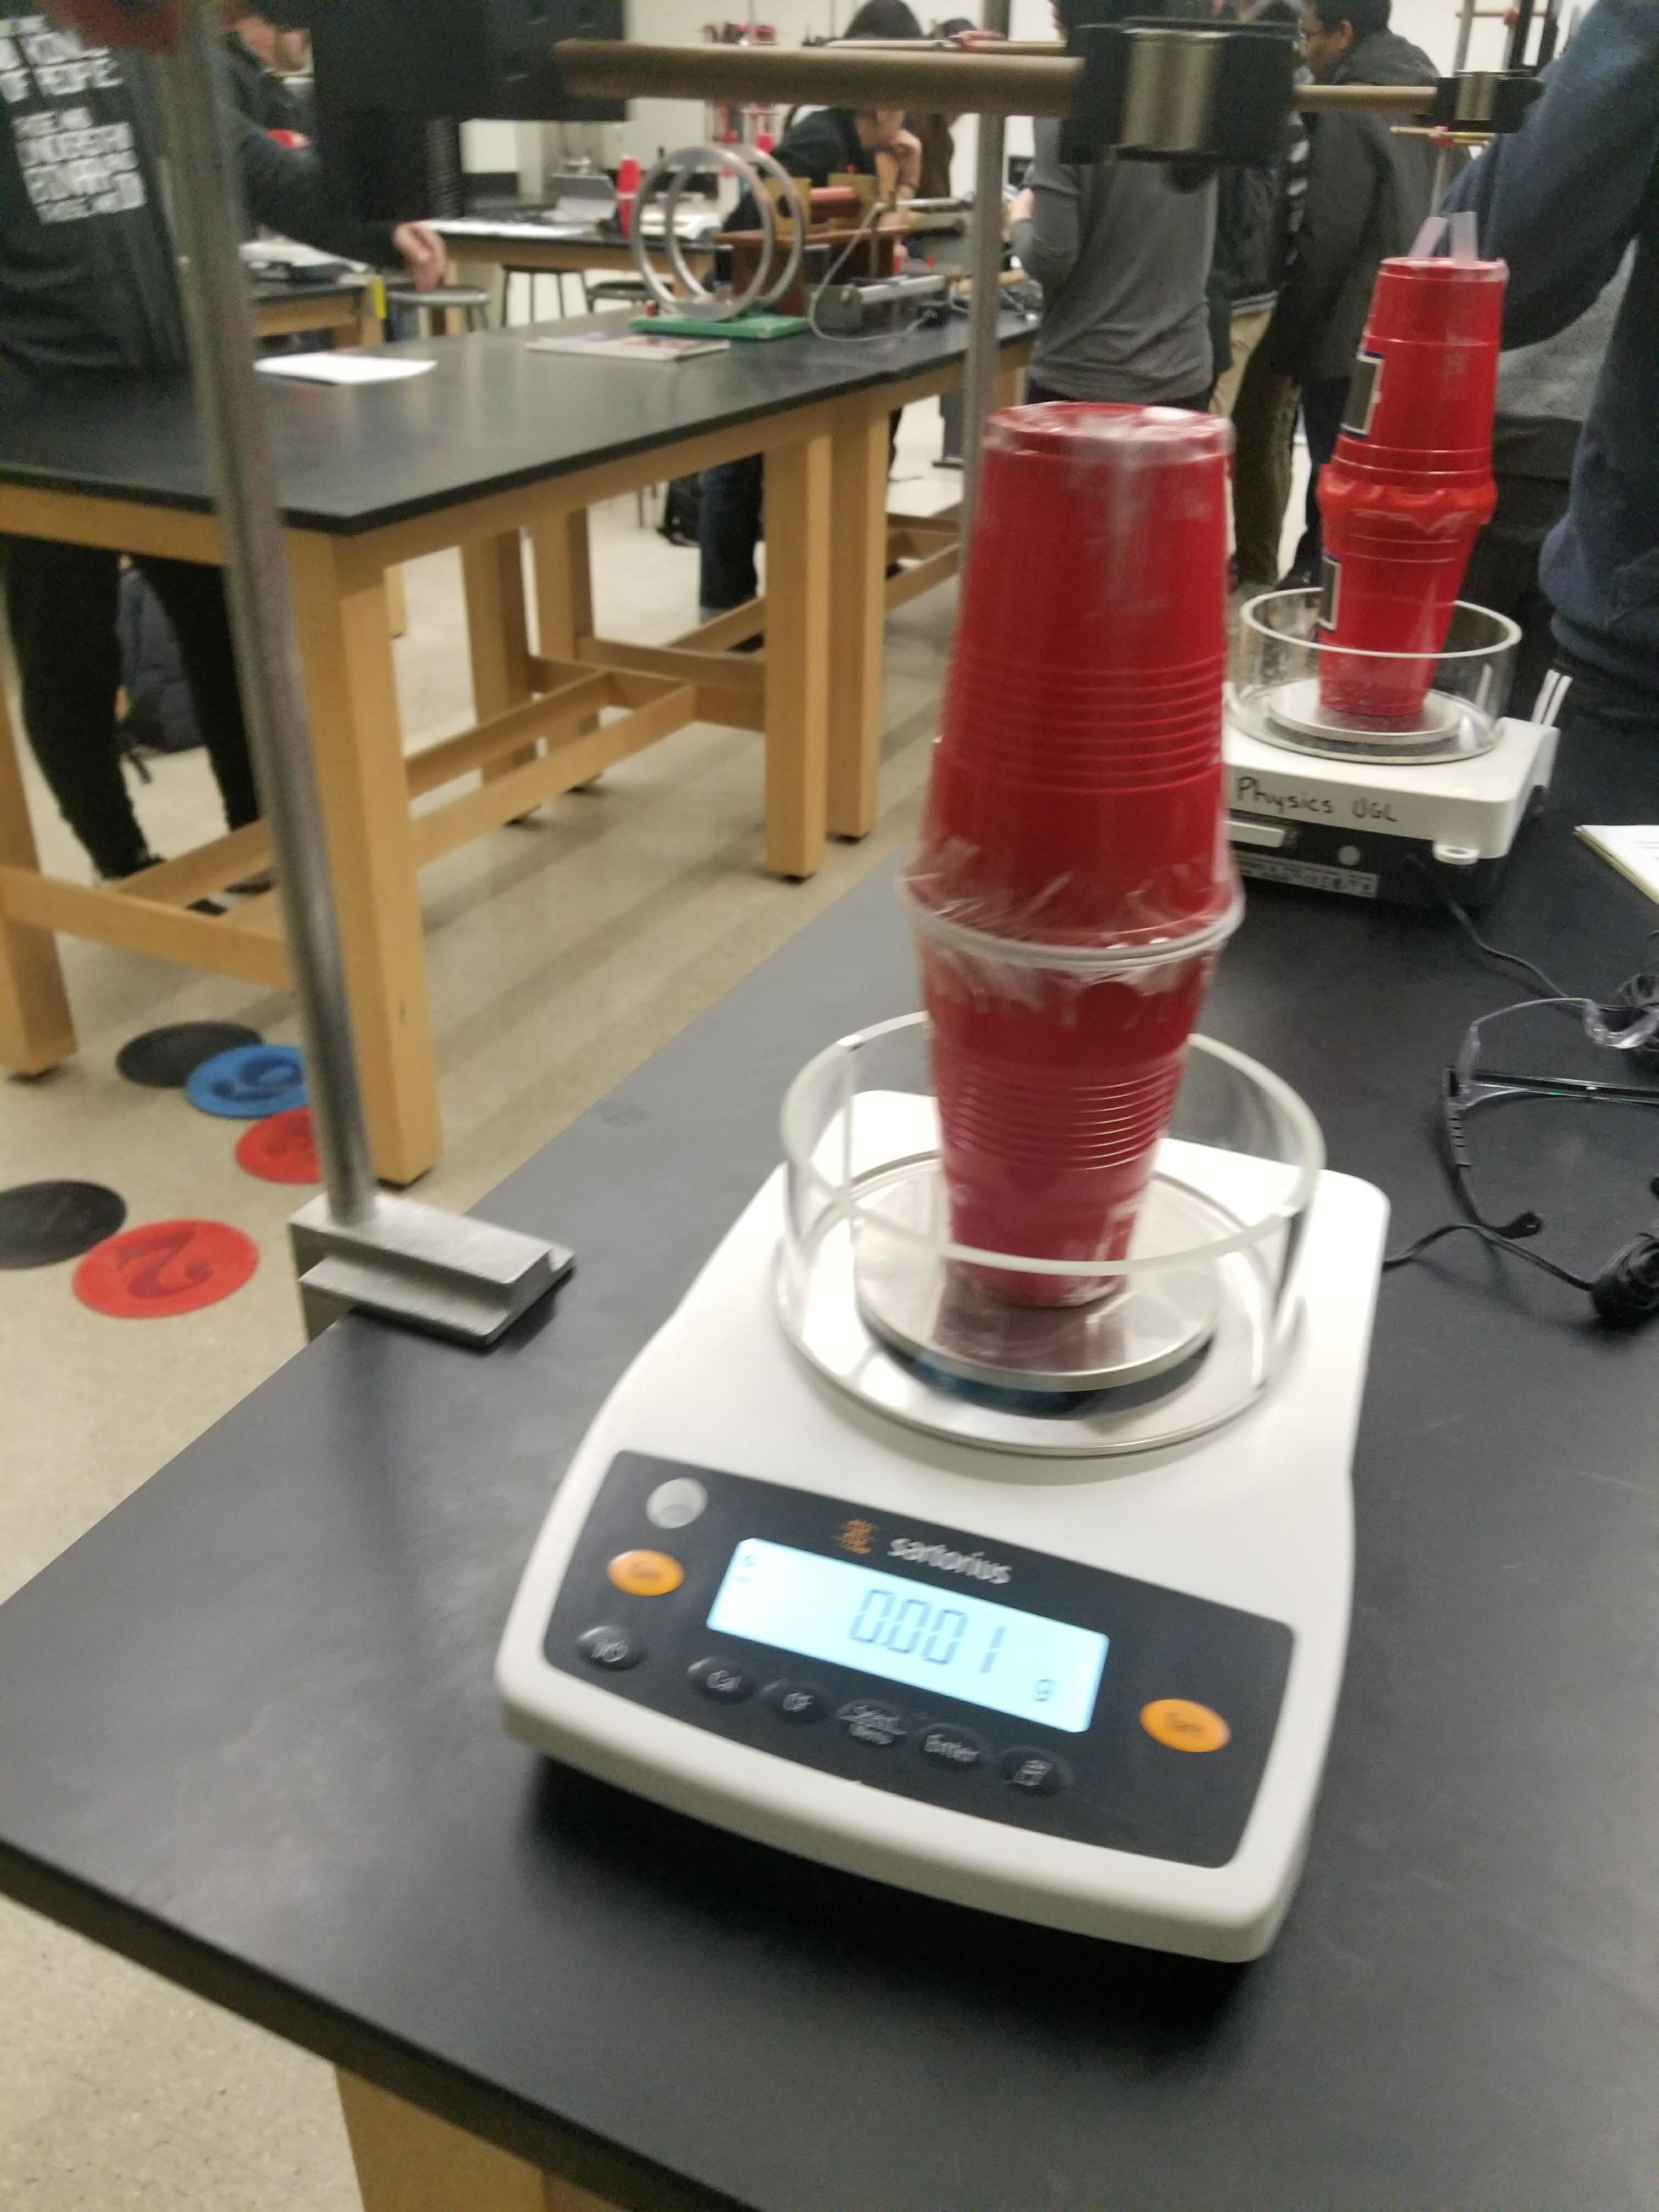
\includegraphics[width=.4\textwidth]{apparatus.jpg}
 \caption{Apparatus used for experiment, along with the electronic balance}
\end{figure}

The experimental setup, as shown in Figure 1 is as follows:
Solo cups taped together are placed on the electronic balance,
and the balance is tared to calibrate its measurement such that
the weight of the cups is not measured. (i.e. only the weight of our
specimens are measured.) For both magnetic materials, an initial reading of the
specimen's weight is taken, which is placed on top of the cups.
The arm is raised as high as possible to keep the strong rare-earth magnet
as far away as possible from the specimen, because at close distances, the reading on the scale
will be skewed, due to the magnetic field of the strong rare-earth magnet.
Then, several measurements are recorded at various distances as the rare-earth magnet is moved towards the
specimen, since the magnetic field of the rare-earth magnet
interacts with the specimen and changes the weight measured by the scale.
The readings on the scale are converted into Newtons, and the distances measured are from the bottom
of the rare-earth magnet to the top of the specimen, measured in metres.


\section{Results}

\subsection{Part 1}

The constants measured and values calculated used to generate Table 2 are
as follows:

\begin{table}[H]
 \centering
 \begin{tabular}{ll}
  Experimental Constants: & Calculated Constants:                               \\ \hline
                          &                                                     \\
  $L =0.280 \pm 0.001m$   & $\mu_0 =\SI{4 \pi e-7}{\tesla \metre \per \ampere}$ \\
  $R =0.0269 \pm 0.003m$  & $\mu_0 N I/2/L = \SI{1.70E-03}{\tesla}$             \\
  $N = 758$               & $R^2 =0.000724m^2$                                  \\
  $I =1A$                 & $x_c - L/2 =0.111m$                                 \\
  $x_c = 0.2505m$         & $x_c + L/2 = 0.391m$                                \\
  $B_e = -0.257mT$        &                                                     \\
 \end{tabular}
 \caption{Experimental and calculated constants}
\end{table}

Table 2 contains the measured values of the magnetic field at verious
positions in the solenoid, as well as calculated theoretical values.

\begin{table}[]
 \centering
 \begin{tabular}{|c|c|c|c|}
  \hline
  Measured B (mT) & x (m) & Corrected  $(B - B_E),\pm 2\%$ (T) & Theory $B_t$ \\ \hline
  0.50            & 0.099 & 7.57E-04                           & 1.03E-03     \\ \hline
  1.40            & 0.119 & 1.65E-03                           & 2.21E-03     \\ \hline
  1.99            & 0.139 & 2.25E-03                           & 2.93E-03     \\ \hline
  2.19            & 0.159 & 2.45E-03                           & 3.18E-03     \\ \hline
  2.26            & 0.179 & 2.52E-03                           & 3.27E-03     \\ \hline
  2.27            & 0.199 & 2.53E-03                           & 3.31E-03     \\ \hline
  2.25            & 0.219 & 2.51E-03                           & 3.33E-03     \\ \hline
  2.25            & 0.239 & 2.50E-03                           & 3.34E-03     \\ \hline
  2.25            & 0.259 & 2.51E-03                           & 3.34E-03     \\ \hline
  2.26            & 0.279 & 2.52E-03                           & 3.33E-03     \\ \hline
  2.25            & 0.299 & 2.51E-03                           & 3.32E-03     \\ \hline
  2.23            & 0.319 & 2.48E-03                           & 3.28E-03     \\ \hline
  2.18            & 0.339 & 2.44E-03                           & 3.20E-03     \\ \hline
  2.02            & 0.359 & 2.28E-03                           & 2.98E-03     \\ \hline
  1.56            & 0.379 & 1.82E-03                           & 2.36E-03     \\ \hline
  0.65            & 0.399 & 9.11E-04                           & 1.18E-03     \\ \hline
 \end{tabular}
 \caption{Raw data recorded while measuring $B_s$ as the Hall probe was moved in 2 centimetre increments.}
\end{table}

Using the data in Table 2, a graph is generated (Figure 4), such that we can compare our
experimental data to a theoretical curve. A sample calculation for the corrected $B-B_E$
is as follows:
$$ B-B_E = 0.5 mT - (-0.257 mT) = 0.757 mT = \SI{7.57e-4}{\tesla}$$
The theoretical $B_t$ was calculated using the Excel template downloaded from eclass.

By inspection of Figure 4 and Table 2, the ratio $\frac{B_t}{B_{exp}}$ can
be calculated, which is used to scale the slope found in Part 2 of the experiment,
which in turn is used to determine the experimental value of $N$, the number of turns in the coil.
$\frac{B_t}{B_{exp}}$ is found by picking two data points in the centre of the plateau:
$${Theoretical: } (0.259, \num{3.43e-3})$$
$${Experimental: } (0.259, \num{2.51e-3})$$
$$\therefore \frac{B_t}{B_{exp}}= \frac{\num{3.43e-3}}{\num{2.51e-3}}=1.33$$
\begin{figure}[H]
 \centering
 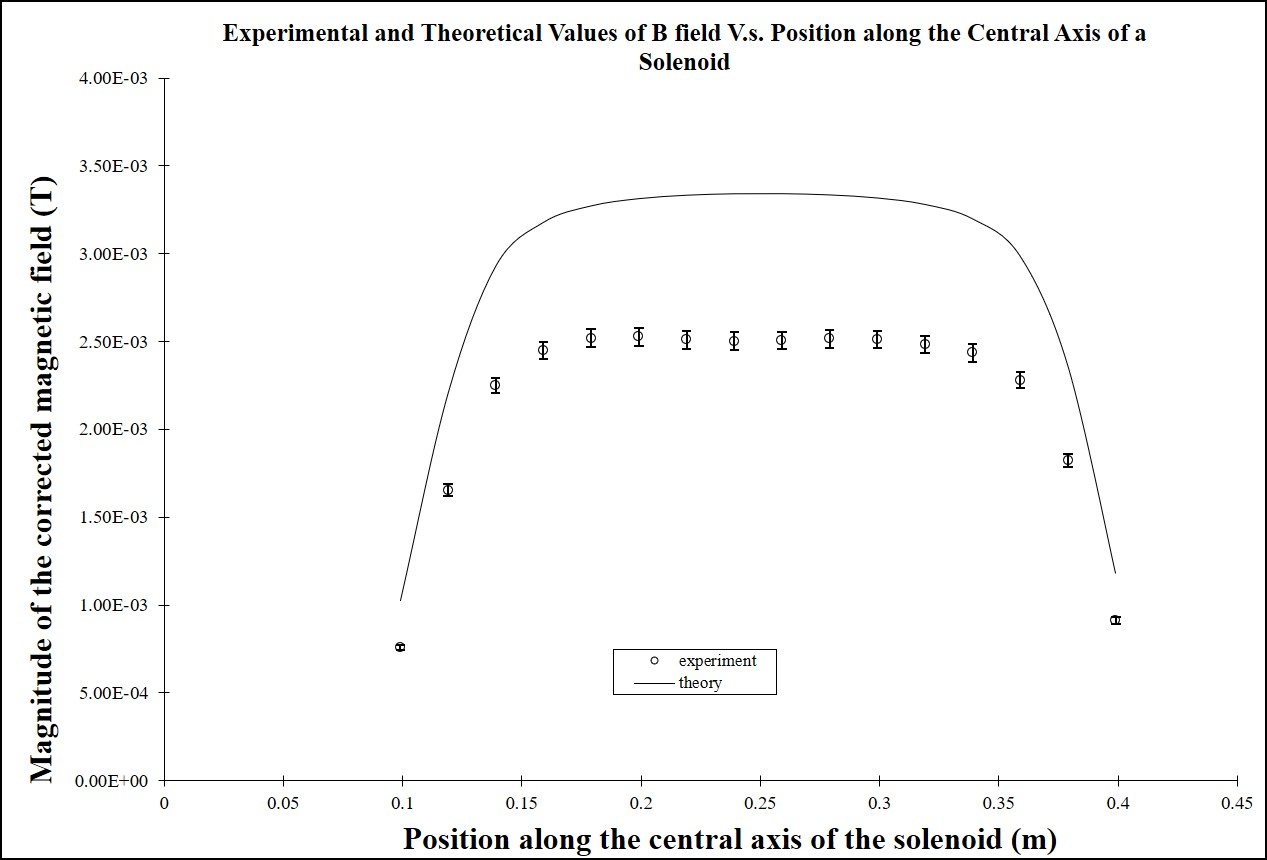
\includegraphics[width=\textwidth]{part1graph.jpg}
 \caption{Experimental values of B field in solenoid compared to theoretical values}
\end{figure}


\subsection{Part 2}

The raw data recorded for part 2 where we beasure $B_H$ in the
Helmholtz coils as a function of current is outlined in Table 2.

\begin{table}[H]
 \centering
 \begin{tabular}{|c|c|}
  \hline
  Current (A) & $B_H (T)$          \\ \hline
  0.1         & -0.000194861519119 \\ \hline
  0.2         & -0.000133962572081 \\ \hline
  0.3         & -6.99808991888E-05 \\ \hline
  0.4         & -1.21344552038E-05 \\ \hline
  0.5         & 4.36568382113E-05  \\ \hline
  0.6         & 0.000108031407536  \\ \hline
  0.7         & 0.000168628126549  \\ \hline
  0.8         & 0.000230010638426  \\ \hline
  0.9         & 0.000286799284324  \\ \hline
  1           & 0.000351052962439  \\ \hline
 \end{tabular}
 \caption{Measured magnitudes of $B_H$ when varying the current in the coil in 0.1A increments}
\end{table}

Given that $R=14.8 \pm 0.2 cm$, we can linearize Equation 3 to
generate a graph (Figure 5), from which we can determine the experimental
value for N  as follows:

$$ B_H = \frac{8\mu_0NI}{\sqrt{125}R} \Rightarrow B_H = N\left( \frac{8\mu_0I}{\sqrt{125}R} \right)  $$
% $$ \therefore B_H = \frac{8 \times \SI{4 \pi e-7}{\tesla\metre\per\ampere}}{\sqrt{125}(\SI{14.8}{\cm})}$$
% $$ \Rightarrow N = \frac{B_H \sqrt{125} R}{8\mu_0I} $$
% $$ \therefore N= \frac{}{} $$
%  so we generate a graph
% with $\frac{\sqrt{2V}}{r}$ on the X axis using our measured voltage values, and $B_H$ on the Y axis
% using our measured current values.
Using the form above, we can plot a graph, such that
$B_H$ is on the y-axis, and $\frac{8\mu_0NI}{\sqrt{125}R}$ is plotted on the x-axis.
Then, our experimental value for N will be the slope, and the y-intercept should theoretically be zero.
\begin{figure}[H]
 \centering
 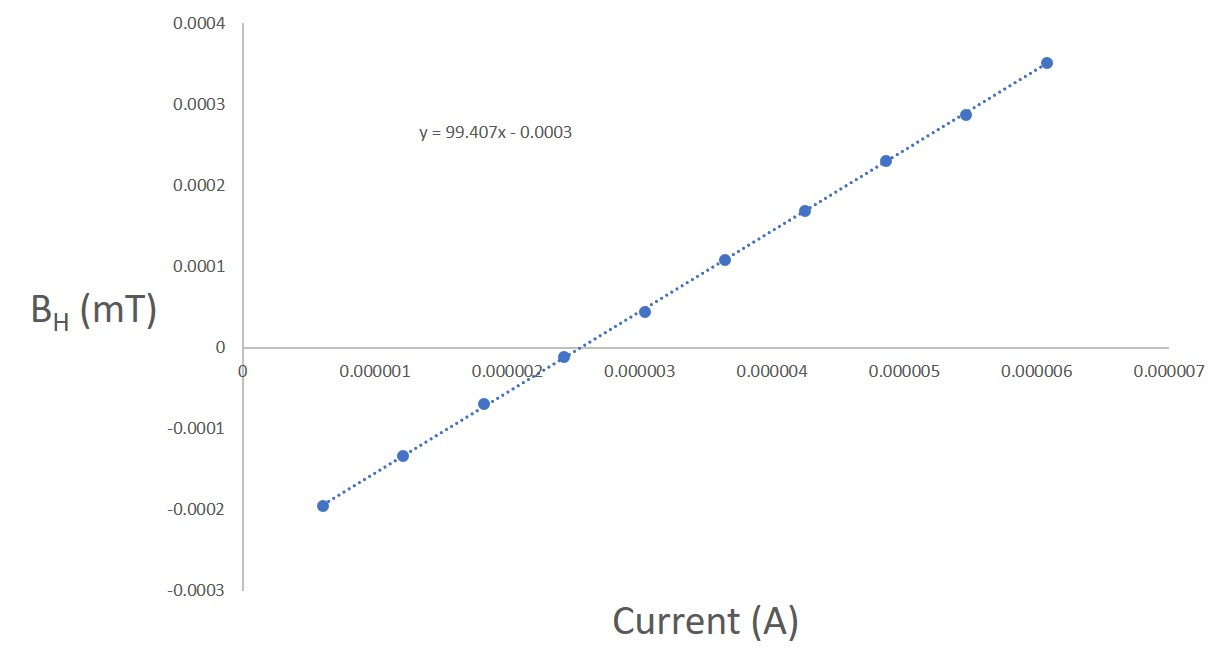
\includegraphics[width=\textwidth]{p2graph.jpg}
 \caption{$B_H$ as a function of current}
\end{figure}

\newpage
\noindent Using Excel's LINEST function, we obtain the following data from the graph in Figure 5.
\begin{table}[H]
 \centering
 \begin{tabular}{cc}
  Slope & $=99.4073706 \pm 0.3873961 $ \\
        & $=99.4 \pm 0.4$
  % Y-Intercept: &  $\num{3.99642631798173E-05}\pm \num{6.40167504007098E-06}$ \\
 \end{tabular}
 % \caption{LINEST data from the graph in Figure 3}
\end{table}

Now, our slope corresponds to N, however to determine our experimental
value for N, we use the scaling factor $\frac{B_t}{B_{exp}}=1.33$ which was
determined in Part 1 of the experiment.

$$ N= 99.4 \times 1.33 \approx 132 \:turns $$
$$ \delta N   = 0.4 \times 1.33 \approx 1 $$
$$ \therefore N = 132 \pm 1 \:turns$$
The theoretical $N=133$

% \vspace{1cm}
% \noindent The calculated values of $e/m$ and $B_E$ from the graph are summarized in Table 3.
% \begin{table}[H]
% \centering
% \begin{tabular}{c|c|c|c|}
%                 & Expected                      & Calculated:                                     & \% Error \\ \hline
% $e/m$: & $\SI{1.76e11}{\coulomb\per\kilogram}$      & $\num{1.70e11} \pm \SI{4.91e9}{\coulomb\per\kilogram}$  &    $3.52$  \\ \hline
% $B_E$: & $4.8 \pm \,\SI{0.3e-5}{\tesla}$           & $\num{4.00e-5} \pm \,\SI{6.40e-6}{\tesla}$                    &   $16.74$  \\ \hline
% \end{tabular}
% \caption{Measured values of $e/m$ and $B_E$ compared to the calculated values obtained from the graph.}
% \end{table}

\section{Discussion}

\subsection{Part 1}

The right hand rule is used to determine the
direction of the magnetic $\textbf{B}$ field in the coils of wire. In the case of the
solenoid, the magnetic field is illustrated in Figure 5 below:

\begin{figure}[H]
 \centering
 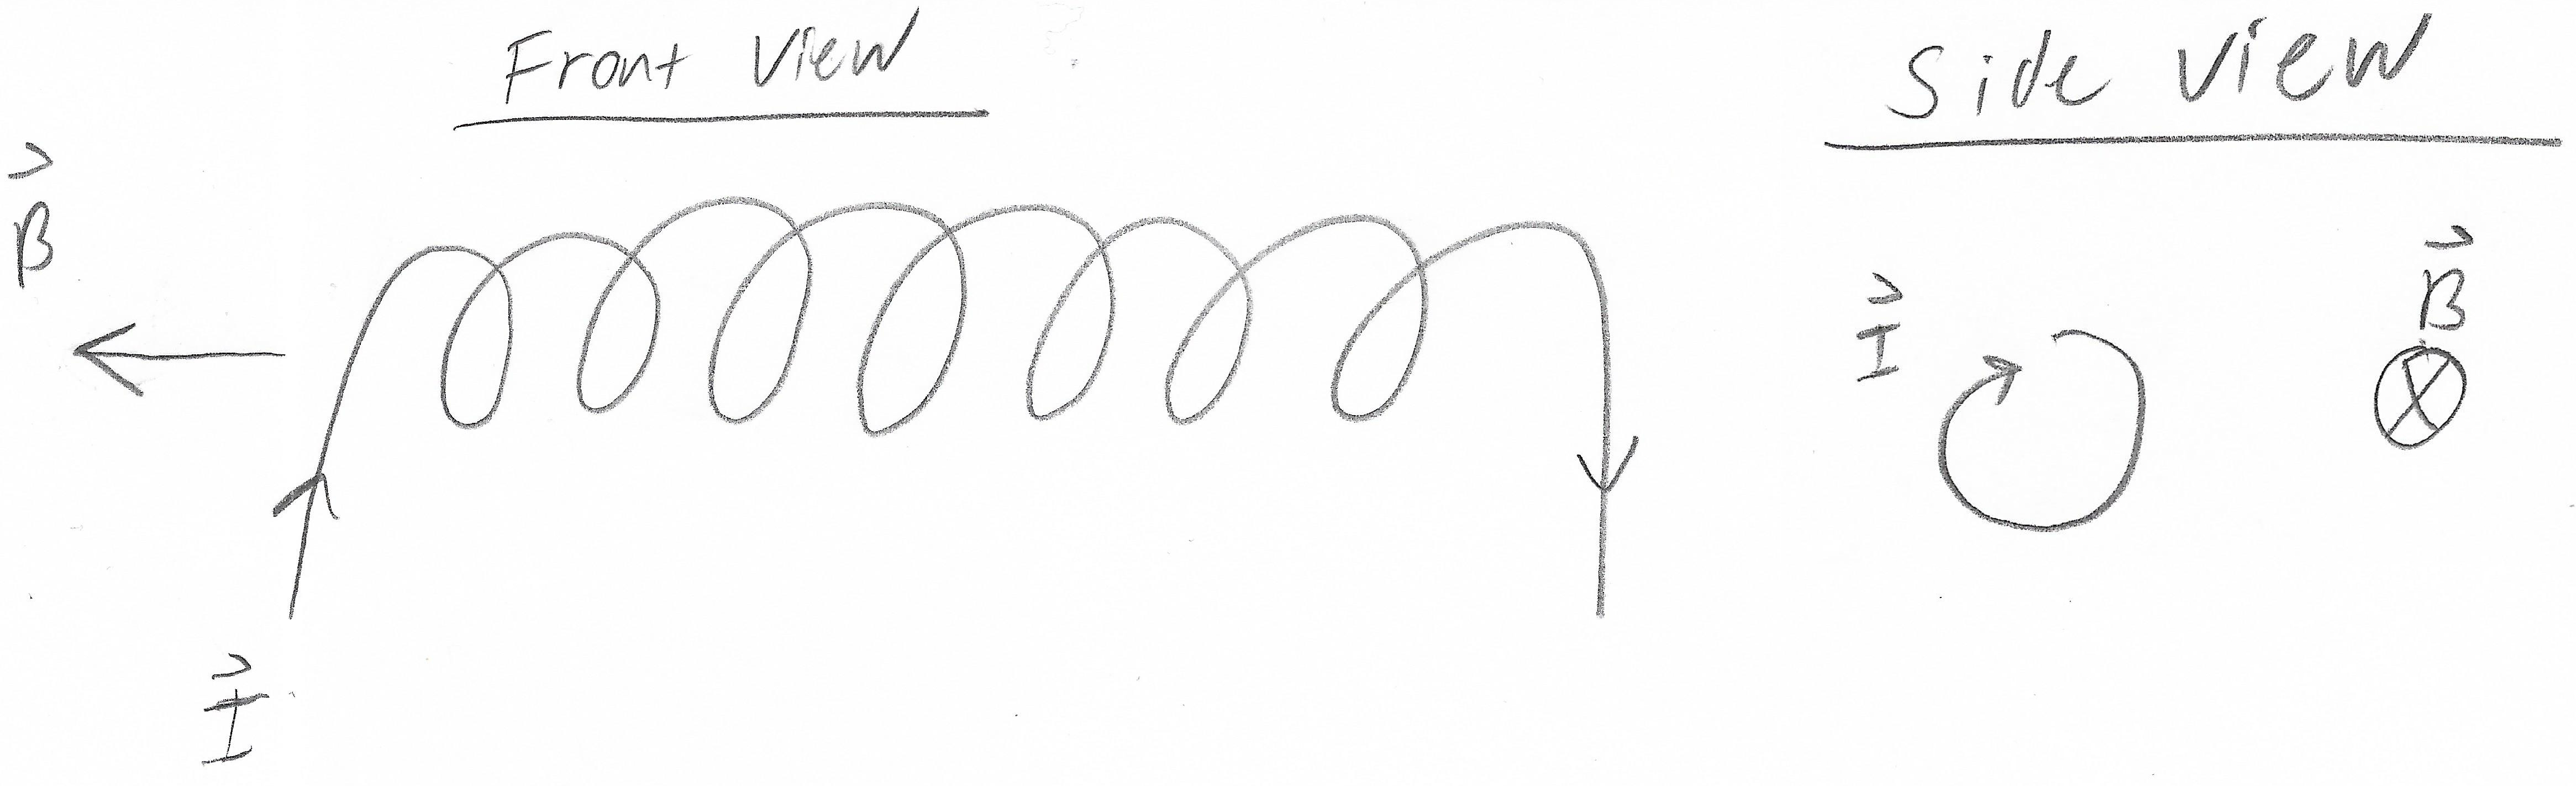
\includegraphics[width=\textwidth]{question1.jpg}
 \caption{Orientation of \textbf{B} vector for a solenoid with current \textbf{I} running through it.}
\end{figure}

From Figure 4, we can see that the experimental values measured are quite different
compared to the theoretical values. However, the shape of both curves are very similar.
In fact, if the experimental values were offset by a scaling factor $\frac{B_t}{B_{exp}}=1.33$ , our
measured results would be extremely close to the expected theoretical curve. Therefore,
the cause of error is constant, which implies that the Hall probe is likely miscalibrated,
or it could be a result of our equations not taking into account the internal resistance of the wires.



\subsection{Part 2}


The graph produced (Figure 5) is linear as expected, with no anomalous data points.
Using the scaling factor 1.33 derived in part 1 of the experiment, we obtain the value $N=132 \pm 1$,
from the slope of the graph in Figure 5, which agrees within error of the theoretical value 133.

% \begin{figure}[H]
%   \centering
%   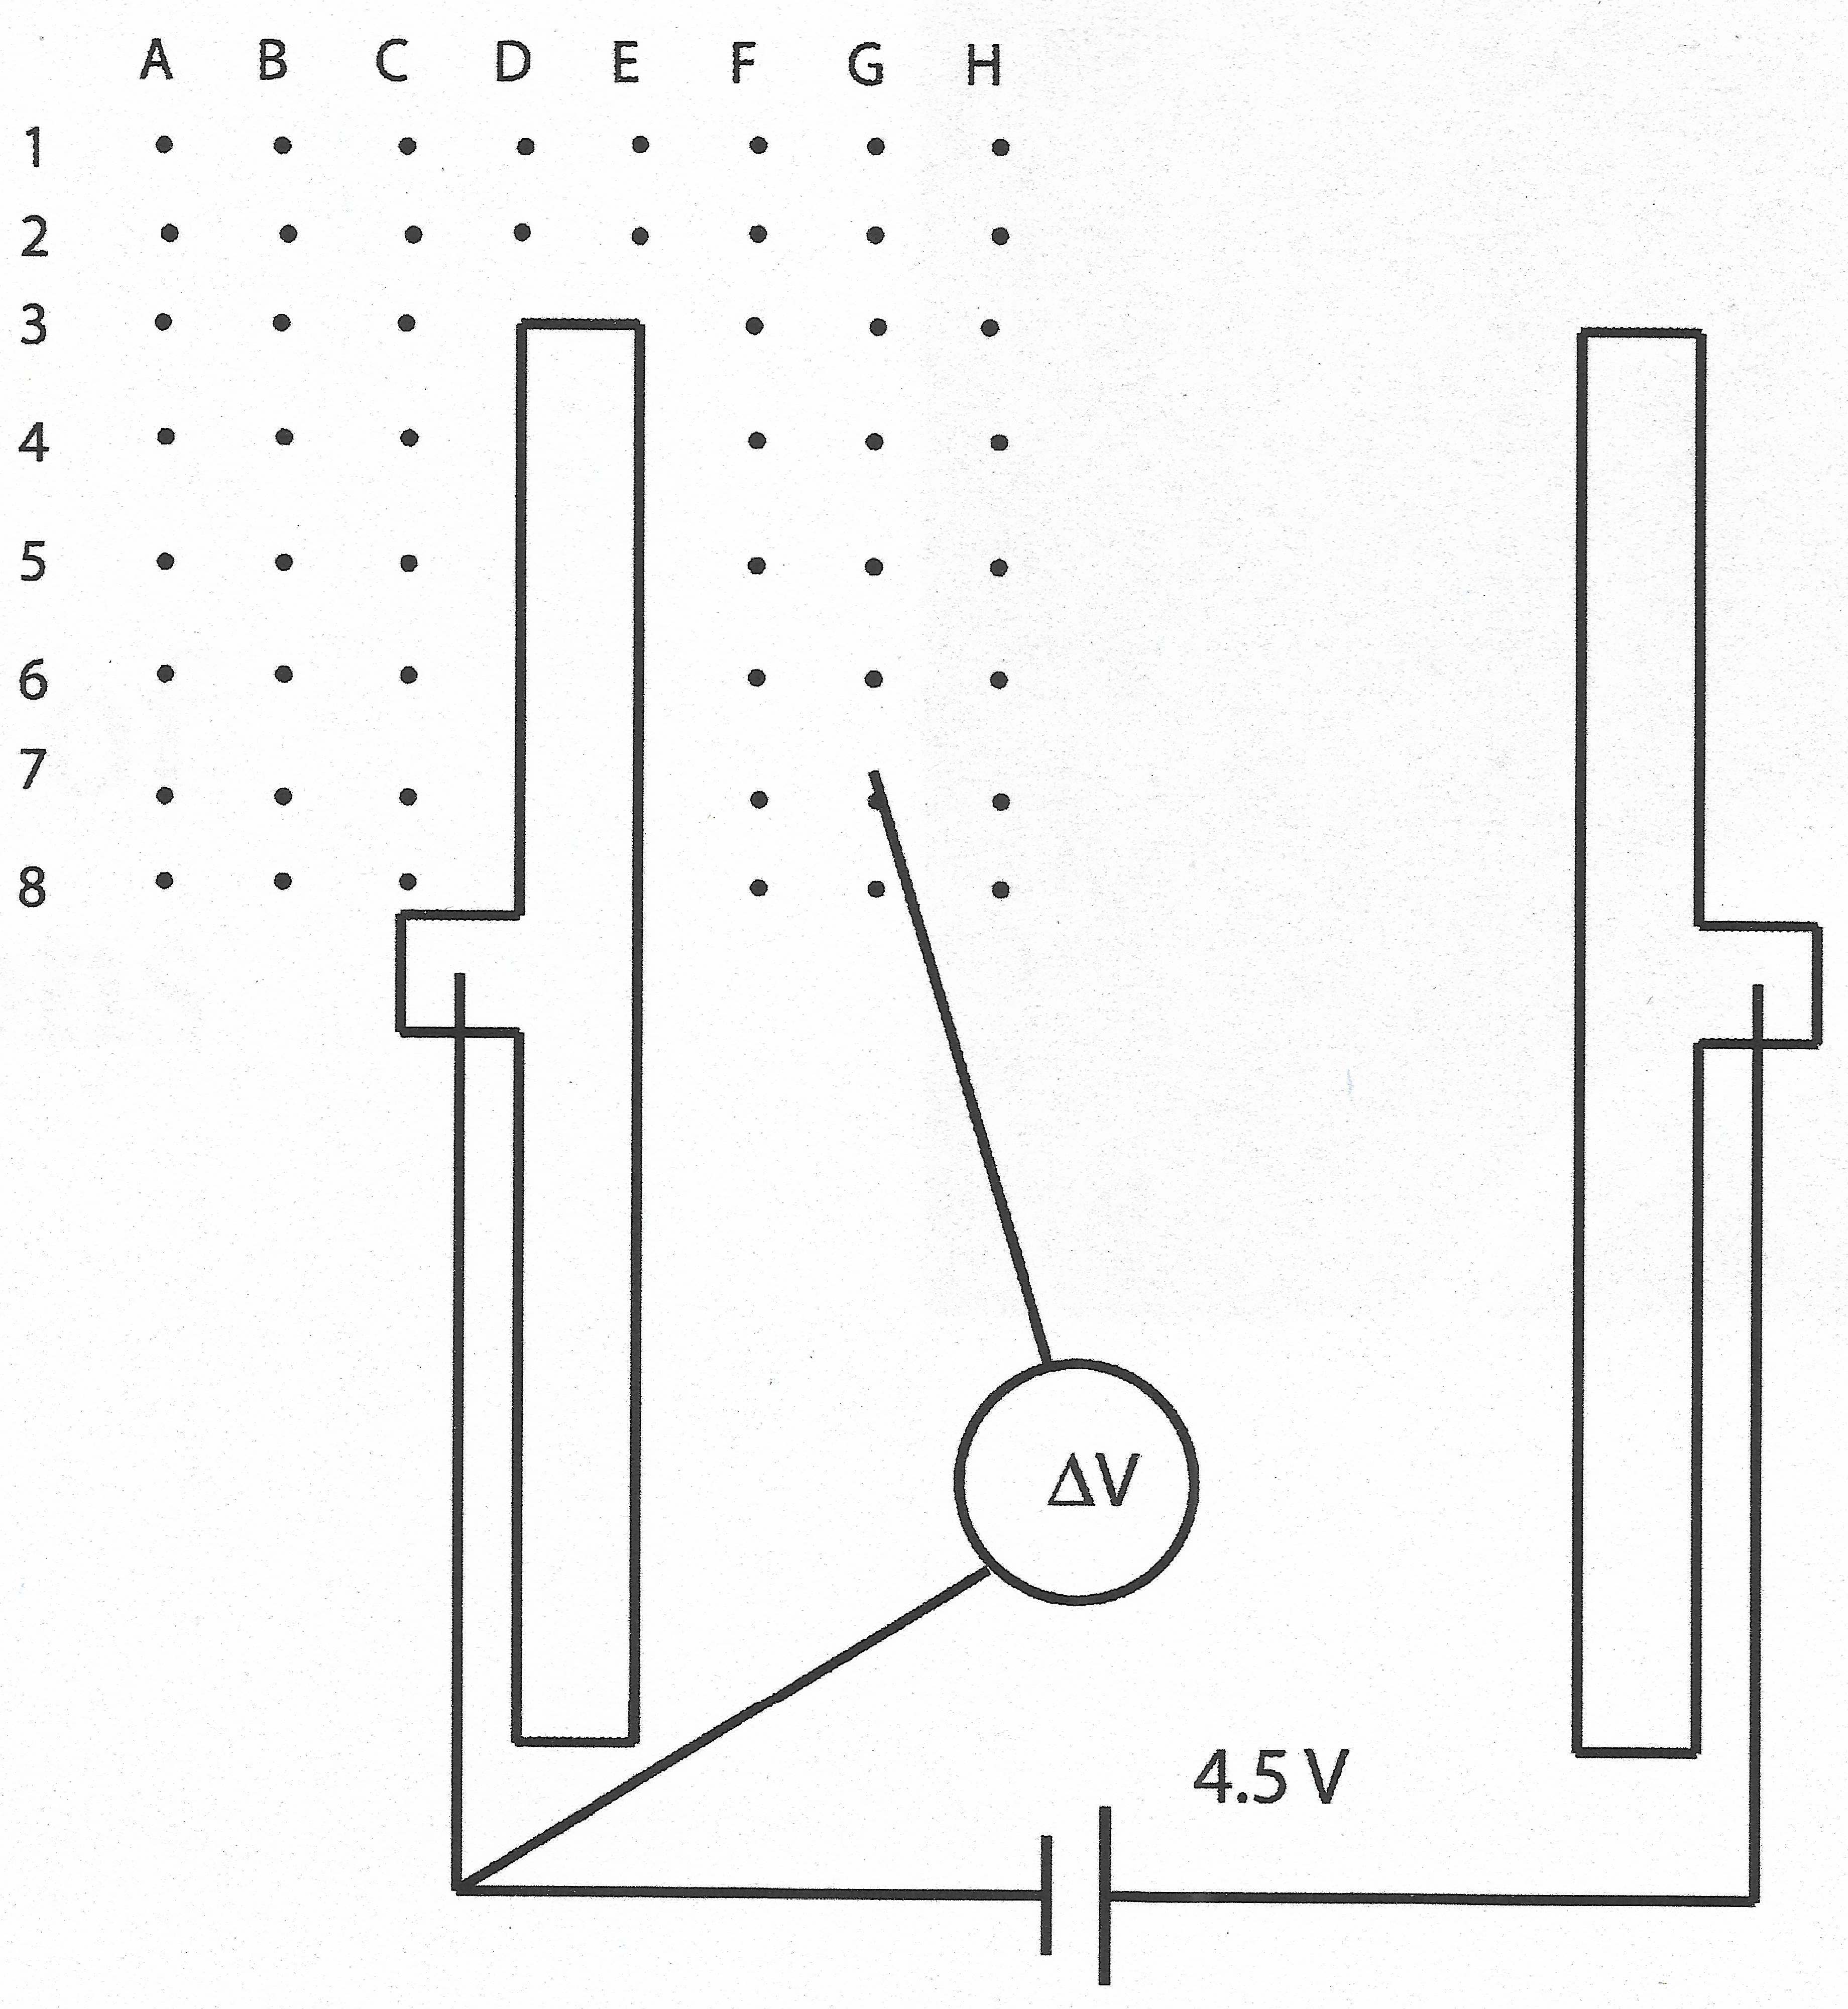
\includegraphics[width=\textwidth]{fig3.jpg}
%   \caption{The direction of the \textbf{B} field is found to be pointing out of the page when drawn this way.}
% \end{figure}

% SOME MORE DERIVATIONS AS FOLLOWS:

Using equation 1, and the geometry from Figure 1, we can find a simplified expression for $B_s$ in the centre of a real solenoid as follows:
$$ \cos{\beta_2} = \frac{L/2}{\sqrt{R^2+L^2/4}}$$
$$ \cos{\beta_1} = \sin{(\pi/2 - \beta_1)} = -\sin{(\beta_1-\pi/2)} = -\frac{L/2}{\sqrt{R^2+L^2/4}}  $$
Substituting into equation 1 yields:
$$ B_s = 1/2 \mu_0nI \left(\frac{L/2}{\sqrt{R^2+\frac{L^2}{4}}} + \frac{L/2}{\sqrt{R^2+\frac{L^2}{4}}} \right) =  1/2\mu_0nI \left(\frac{L}{\sqrt{R^2+\frac{L^2}{4}}} \right)= \frac{\mu_0nIL}{\sqrt{4R^2+L^2}}$$
Since $n=N/L$, we can substitute $nL=N$ to finally obtain:
$$ B_s= \frac{\mu_0NI}{\sqrt{4R^2+L^2}} $$
%and compare it to the
%expected value of 133. The radius of each coil is $14.8\pm 0.2cm$

We can also find an expression for $B_c$ in the centre of a single coil using Equation 2 as follows:\\
At the centre of the coil, $x=x_c$ to obtain:
$$ B_c = \frac{\frac{1}{2} \mu_0NR^2I}{(R^2+(x_c-x_c)^2)^{3/2}} $$
which simplifies nicely:
$$ \frac{\frac{1}{2} \mu_0NR^2I}{(R^2)^{3/2}} = \frac{\frac{1}{2} \mu_0NR^2I}{R^3}  $$
$$ \therefore B_c = \frac{\frac{1}{2} \mu_0NI}{2R} $$

Additionally, the expression for $B_H$ can be obtained from the expression for $B_c$ derived above. By inspection,
we notice that $x-x_c=R/2$, which we can substitute into Equation 2 to obtain:
$$ B_c= \frac{\frac{1}{2}\mu_0NR^2I}{(R^2+(\frac{R}{2})^2)^{3/2}} = \frac{\frac{1}{2}\mu_0NR^2I}{\frac{\sqrt{125}}{8}R^3} = \frac{1}{2}\times \frac{8\mu_0NI}{\sqrt{125}R} $$
and by realizing that $2B_c=B_H$, we finally obtain Equation 3 by multiplying the above expression by 2:
$$B_H=\frac{8\mu_0NI}{\sqrt{125}R}$$
\section{Conclusions}

In Experiment 2, we measure the distribution of the magnetic field across a solenoid,
and we also measure the magnetic field of a Helmholtz coil from which we experimentally determine the
number of turns of the wire in the coil. In the first part, a Hall probe was used to measure the magnetic field
at various points inside a solenoid. The graph produced from our experimental values
closely matched the shape of the theoretical curve, even though the measured values were
quite different from the theoretical values. If each recorded
data point was scaled by 1.33, the measured values would fit the
theoretical curve very nicely, which implies that the Hall probe
was likely miscalibrated, or some factor was not being taken into account such as the internal resistance
of the wires. In part 2, the Hall probe was used to measure the magnetic field
at the center of the Helmholtz coils with varying current, from which we could experimentally
determine the number of turns of the wire in the coils by plotting a graph, and using the scaling factor obtained in Part 1
to correctly determine the number of turns in the Helmholtz coil by multiplying the slope of our graph by 1.33. The measured value was $132 \pm 1$ turns, which agrees
within error of the expected value of 133 turns.

\bibliography{references}
\end{document}
